\section{Parte 1: Análisis dinámico del pozo infinito simétrico [45 puntos]}


\begin{pregunta}{1.}
\textbf{Cálculo de las amplitudes.} Aplicando la condición de normalización $\int_{-\infty}^{\infty} |\varphi_n(x)|^2 \, \mathrm{d}x = 1$, demuestren \textbf{analíticamente} que las amplitudes $A_n$ y $B_n$ en los eigenestados pares e impares del pozo finito simétrico están dadas por las Ecs. 18 y 19

\begin{equation}
A_n = \sqrt{\frac{q_n}{a q_n + 1}}, \qquad B_n = \frac{\cos k_n a}{\exp(-q_n a)} A_n, \tag{18}
\end{equation}
donde $k_n = (\pi/2a)\,\mu_n$ y $q_n = (\pi/2a)\sqrt{\mu_{\text{máx}}^2 - \mu_n^2}$. Para los eigenestados impares obtenemos
\begin{equation}
A_n = \sqrt{\frac{k_n}{a k_n - \tan(a k_n)}}, \qquad B_n = \frac{\sin k_n a}{\exp(-q_n a)} A_n. \tag{19}
\end{equation}
\end{pregunta}
%================================================================================
% INICIO PREGUNTA 1

El pozo finito simétrico tiene la siguiente función de potencial.
\begin{equation*}
U\left(x\right)=\left\{\begin{array}{ll}0, & \left|x\right|<a\\ U_0, & \left|x\right|>a\end{array}\right., \qquad U_0\in\mathbb{R}>0.
\end{equation*}

Para este pozo en particular, tenemos las siguientes soluciones dependiendo del intervalo en función de $k_n$ y $q_n$. Por ahora, analicemos los eigenestados pares.  
\textbf{Eigenestados pares} (simétricos)
\begin{equation*}
\varphi_n\left(x\right)=\left\{\begin{array}{lll}A_n\cos k_n x, & \left|x\right|<a, \qquad & k_n=\sqrt{2ME_n/\hbar^2},\\ B_n\exp\left(-q_n x\right), & x>a, \qquad & q_n=\sqrt{2M\left(U_0-E_n\right)/\hbar^2}.\end{array}\right.
\end{equation*}

Se inicia con la condición de normalización, que implica que la partícula debe estar en algún lugar en todo el espacio... 

\begin{equation}
    1 = \int_{-\infty}^{-a}B_n^2 \exp (2q_nx) \, dx 
    + \int_a^{\infty} B_n^2 \exp (-2q_nx) \, dx
    +2A^2_n \int_0^a\cos^2 (k_nx) \,dx
    \label{eq: norm:prob}
\end{equation}


Por simetría, las primeras dos integrales de ecuación \ref{eq: norm:prob} son simétrica y juntas dan un resultado de $B_n^2/q_n \exp (-2q_n a)$, mientras que la última integral se resuelve usando la identidad $\cos^2(k_nx)=\frac{1}{2}(1+\cos(2k_nx))$. Por lo que ecuación \ref{eq: norm:prob} se simplifica a:

\begin{equation}
    1= \frac{B^2_n}{q_n} \exp (-2q_na)+A_n^2\left(a+\frac{1}{2k_n}\sin(2ak_n)\right)
    \label{eq: A y B prob1}
\end{equation}


Para simplificar esto, se necesita una relación entre la variable $B_n$ y $A_n$. Dado que $\varphi_n$ debe ser continua, ambos deben valer lo mismo en $x=a$. Por lo que:

\begin{equation}
    A_n\cos(k_na)=B_n \exp(-q_na)
    \label{eq: cond front1}
\end{equation}

Ahora se reescribe \ref{eq: A y B prob1} en función de $A_n$ y se busca resolver para $A_n$.

\begin{align}
    1=&A_n^2\left(\frac{\cos^2(k_na)}{q_n}+a+\frac{1}{2k_n}\sin(2ak_n)\right) \\
    A_n^2 &= \frac{1}{\frac{\cos^2(ak_n)}{q_n} + a+\frac{1}{2k_n}\sin(2ak_n)}
\end{align}

Multiplicando por $q_n$ y utilizando la ecuación característica $\tan(ak_n)=\frac{q_n}{k_n}$, se puede llegar a la siguiente ecuación:

\begin{align}
    A_n^2 =& \frac{q_n}{\cos^2(k_na)+q_na+\sin^2(k_na)} \\
    A_n =& \sqrt{\frac{q_n}{1+q_na}} \label{eq: A par}
\end{align}

Donde la ecuación \ref{eq: A par} nos da el valor de $A_n$ para que este sea siempre normalizado. Ahora, para obtener $B_n$ se utiliza la ecuación \ref{eq: cond front1} y se llega a:
\begin{equation}
    B_n=\frac{\cos(k_na)}{\exp(-q_na)}A_n
\end{equation}

Ahora, se continua con los estados impares. 

\begin{itemize}
    \item \textbf{Eigenestados impares} (antisimétricos)
    \begin{equation}
        \varphi_n\left(x\right) = \left\{
        \begin{array}{lll}
            A_n \sin k_n x, & \qquad |x| < a, & \qquad k_n = \sqrt{2ME_n/\hbar^2}, \\
            B_n \exp\left(-q_n x\right), & \qquad x > a, & \qquad q_n = \sqrt{2M\left(U_0 - E_n\right)/\hbar^2}.
        \end{array}
        \right.
    \end{equation}
\end{itemize}

\textbf{Nota:} en la fuente original las definiciones de $k_n$ y $q_n$ para los eigenestados impares aparecen intercambiadas. Aquí se corrigen para que coincidan con las de los eigenestados pares, ya que $k_n$ corresponde a la región $|x|<a$ donde $U=0$, y $q_n$ a la región $|x|>a$ donde $U=U_0$.

Se inicia nuevamente con la condición de normalización, que lleva a:

\begin{equation}
    \frac{1}{2} = \int_0^a A_n^2 \sin^2(k_nx) \, dx + \int_a^{\infty} B_n^2 \exp(-2q_nx) \, dx
\end{equation}

\begin{equation}
    \frac{1}{2} = \frac{1}{2}\left[A_n^2 \int_0^a \left(1-\cos(2k_nx)\right) dx + \frac{B_n^2}{q_n}\exp(-2q_nx)\Big|_{\infty}^{a}\right]
\end{equation}

\begin{equation}
    1 = A_n^2\left[a-\frac{\sin(2k_na)}{2k_n}\right] + \frac{B_n^2}{q_n}\exp(-2q_na)
    \label{eq: norm impar}
\end{equation}

Ahora, se usa nuevamente la condición de frontera:

\begin{equation}
    A_n\sin(k_na) = B_n\exp(-q_na)
    \label{eq: cond front impar}
\end{equation}

Por lo que ahora en términos de $A_n$ \ref{eq: norm impar} se vuelve:

\begin{align}
    1 =& A_n^2\left[a-\frac{\sin(2k_na)}{2k_n}+\frac{\sin^2(k_na)}{q_n}\right] \\
    A_n^2 =& \frac{1}{a-\frac{\sin(2k_na)}{2k_n}+\frac{\sin^2(k_na)}{q_n}}
    \label{eq: A2 impar}
\end{align}

Para simplificar \ref{eq: A2 impar} se utiliza la ecuación maestra:

\begin{equation}
    \cot(k_na) = -\frac{q_n}{k_n}
    \label{eq: ec maestra impar}
\end{equation}

Usando \ref{eq: ec maestra impar} y multiplicando por $q_n$ \ref{eq: A2 impar}, se llega a:

\begin{align}
    A_n^2 =& \frac{q_n}{aq_n+\cos^2(k_na)+\sin^2(k_na)} \\
    A_n =& \sqrt{\frac{q_n}{aq_n+1}} \label{eq: A impar}
\end{align}

Por lo que $B_n$ llega de \ref{eq: cond front impar}:

\begin{equation}
    B_n = \frac{\sin(k_na)}{\exp(-q_na)}A_n
    \label{eq: B impar}
\end{equation}

Quedando entonces demostrado el cálculo de las amplitudes.


 %================================================================================
\begin{pregunta}{2.}
\textbf{Cálculo de las eigenenergías y estados estacionarios.} Elabora una rutina computacional para encontrar las eigenenergías $E_n$ en un pozo finito. Para fines numéricos, consideren las constantes $\hbar = 1$, semi-ancho del pozo $a = 1$, y masa $M = \pi^2/8$. Estos valores están pensados para que la energía basal del pozo infinito [Ec. (15)] sea $V_0 = 1$. Como ejemplo concreto, para la profundidad del pozo toma $U_0 = 110$.
 
Programa una función que evalúe los eigenestados $\varphi_n(x)$ del pozo finito.
 
\textbf{Para el reporte:}
 
$\rightarrow$ Tabulen los valores de todas las energías permitidas en el pozo.
 
$\rightarrow$ Grafiquen los primeros 8 eigenestados $\varphi_n(x)$ del pozo. Corroboren que entre más grande es la energía, el eigenestado penetra más en la región clásicamente \textit{prohibida}, es decir, donde $|x| > a$. Asegúrense de usar las amplitudes $A_n$ y $B_n$ analíticas para que sus eigenestados estén normalizados automáticamente. Para tener un indicio de que las cosas están correctas, verifiquen usando diversas parejas de eigenestados que se cumple la ortonormalidad
\begin{equation}
\int_{-\infty}^{\infty} \varphi_p^{*}(x) \, \varphi_q(x) \, \mathrm{d}x = \delta_{pq}. \tag{1}
\end{equation}
Esta integral puede hacerse con la regla del trapecio si muestrean la coordenada $x$ con suficiente resolución y tomando un intervalo lo suficientemente grande para asegurarse que las exponenciales han decaído prácticamente a cero. Así el error de truncamiento es despreciable.
\end{pregunta}

\subsection*{Sobre el código:}

El código se puede ver en el apéndice. Véase el Apéndice \ref{ap: sec1prob2}. Ahora sí, continuemos con el problema.
\\ 

Primero, se muestra en la Tabla \ref{tab:energies} los distintos valores de las energías encontrados al resolver la ecuación maestra. Como el pozo es finito, hay un finito de energías permisibles para estados atrapados. En este caso, se obtienen $11$ eigenenergías. 
\begin{table}[h]
\centering
\begin{tabular}{cccc}
\hline
$n$ & Even energies & $n$ & Odd energies \\
\hline
1 & 0.8887 & 2& 3.5531 \\
3 & 7.9880 & 4& 14.1841 \\
5 & 22.1268 & 6& 31.7943 \\
7 & 43.1531 & 8& 56.1502 \\
9 & 70.6928 & 10& 86.5879 \\
11 & 103.2200 &--& -- \\
\hline
\end{tabular}
\caption{Tabulación de los estados de energía para los estados tanto pares e impares. Se muestra en este caso 6 energías para los estados pares y 5 para los impares.}
\label{tab:energies}
\end{table}


Asimismo, en la Figura \ref{fig:eigenenergies}, se puede ver de una forma gráfica las energías, en comparación al pozo finito. Se observa que al inicio, están muy juntas mientras que las últimas están muy cerca del fin del pozo. 

Se espera que los eigenestados con energías bajas se parezcan a los eigenestados del pozo infinito, mientras que los eigenenergias con energías altas tengan una alta penetración en el pozo.
\begin{figure}
    \centering
    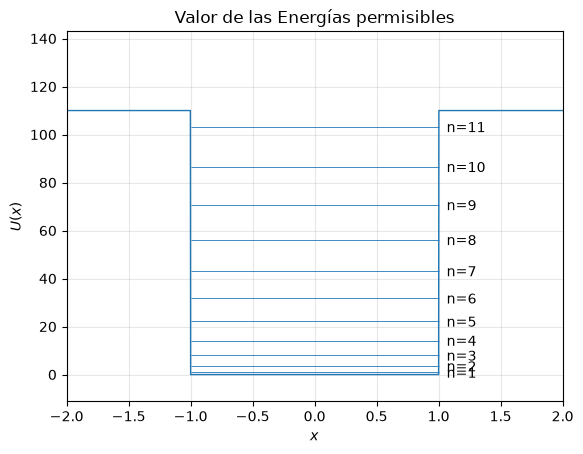
\includegraphics[width=0.75\linewidth]{mini1/energiaspermisibles.png}
    \caption{Se muestran como rayas todas las energías permitidas en el pozo. Para los valores específicos de $a=1, U_0=110, V_0=1, M=\frac{\pi^2}{8}$, obtuvieron 11 energías. Se observa que la separación entre cada energía va aumentando conforme aumenta el nivel.}
    \label{fig:eigenenergies}
\end{figure}

En la Figura \ref{fig:eigenestados}, se pueden observar los primeros 8 eigenestados del pozo finito. Como se esperaba, los primeros eigenestados, se parecen al pozo infinito, dado que casi no se llega a penetrar la pared. En cambio, los estados grandes este efecto es más notorio. Ahora, lo último que queda es checar la ortonormalidad de las ecuaciones. Se realiza la siguiente integral de manera computacional:

\begin{equation}
\int_{-\infty}^{\infty} \varphi_p^{*}(x) \, \varphi_q(x) \, \mathrm{d}x = \delta_{pq}. 
\label{eq:ortonormality}
\end{equation}
\begin{figure}
    \centering
    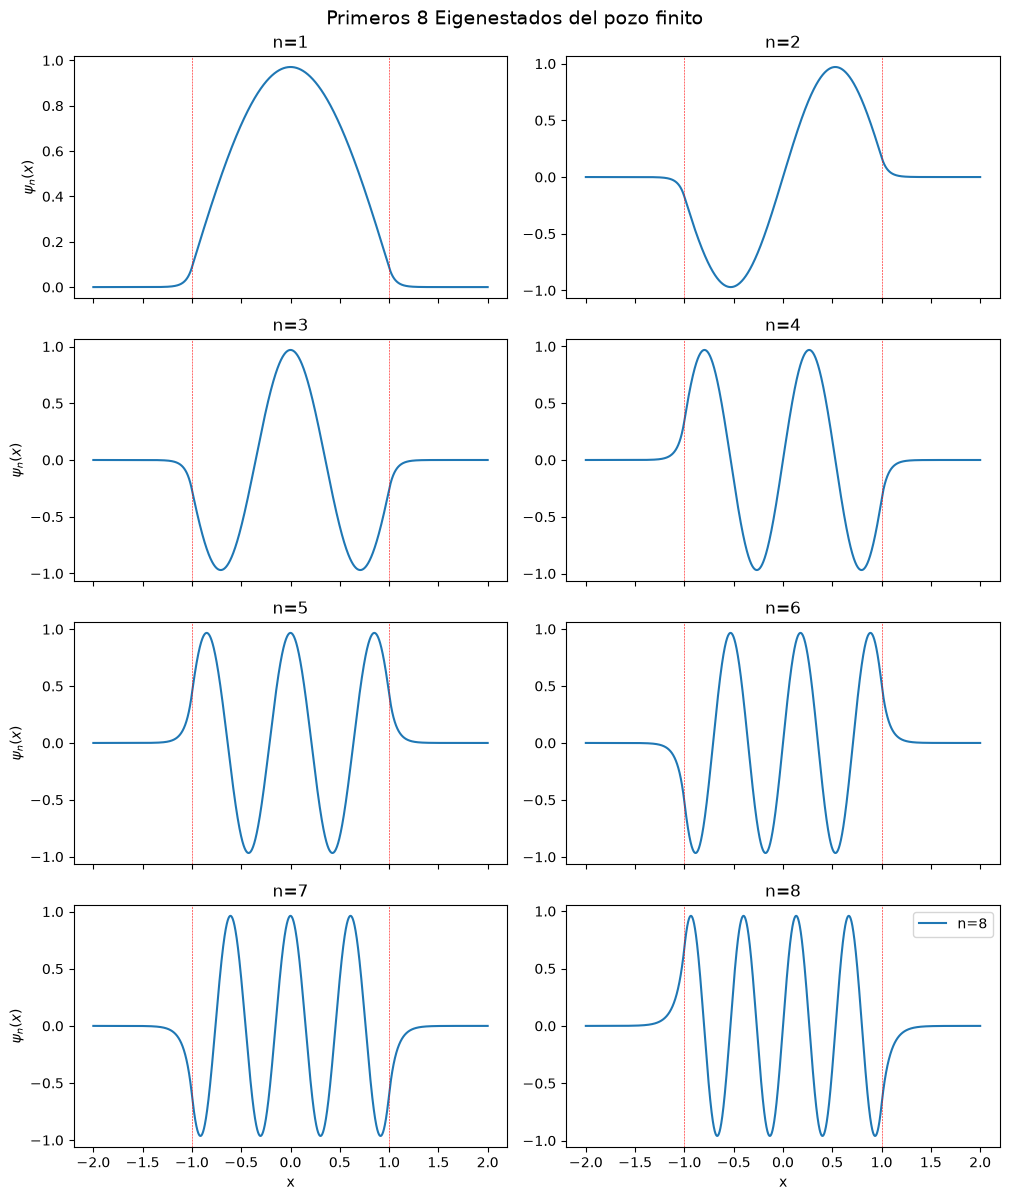
\includegraphics[width=0.75\linewidth]{eigenestados.png}
    \caption{Los eigenestados de las primeras 8 energías del pozo. Se observa que están todas entre el rango de -1 a 1, que debe ser así para ser normalizadas. En la región del pozo, se muestran oscilaciones de senos o cosenos, mientras que después del pozo se observan exponenciales por la zona prohibida. Para energías altas, se llega a penetrar más en la zona prohibida.}
    \label{fig:eigenestados}
\end{figure}


Ahora, para poder ver que realmente los eigenestados son ortonormales, utilizamos una matriz de traslape $S$ en el cual sus entradas se definen de la siguiente manera:

\begin{equation}
    S_{ij} = \int_{-\infty}^{\infty} \varphi_i^{*}(x) \, \varphi_j(x) \, \mathrm{d}x
\end{equation}

El resultado de $S$ se puede apreciar en la Figura \ref{fig:overlaps}. Claramente aquí se demuestra la ortogonalidad dado que representa una matriz identidad, que es equivalente a la delta de Dirac que se utiliza en la ecuación \ref{eq:ortonormality}.


\begin{figure}
    \centering
    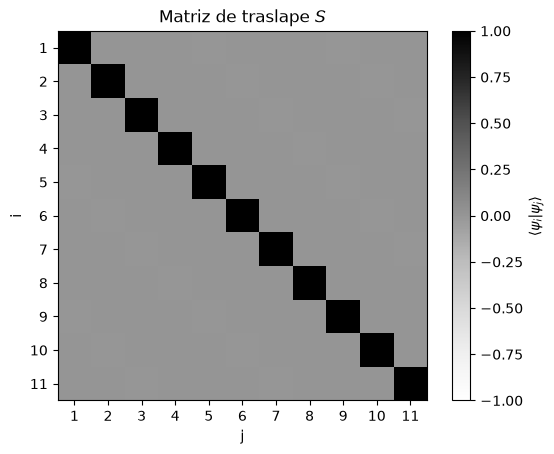
\includegraphics[width=0.75\linewidth]{overlapS.png}
    \caption{La matriz de traslape $S$ que muestra la ortonormalidad de los eigenestados. Como solamente la diagonal principal contiene valores no nulos, se muestra la ortogonalidad. Asimismo, como esta tiene una diagonal de 1's, vemos que está también normalizada y por lo tanto los eigenestados son ortonormales.}
    \label{fig:overlaps}
\end{figure}





 
\begin{pregunta}{3.}
\textbf{Evolución temporal.} En el problema anterior hemos encontrado la base de eigenestados ortogonales del pozo finito, las funciones $\varphi_n(x)$, donde $n = \{1, 2, \ldots, N\}$ con $N$ siendo el máximo número de eigenestados atrapados en el pozo. Programen una rutina computacional para simular la evolución temporal de una función de onda inicial $\phi(x,0) = f(x)$ dentro del pozo finito de potencial. Como base del algoritmo, usen la expansión estándar en términos de eigenestados
\begin{equation}
\phi(x,t) = \sum_{n=1}^{N} c_n \varphi_n(x) \exp(-\mathrm{i}\omega_n t), \qquad \omega_n = \frac{E_n}{\hbar}, \tag{2}
\end{equation}
donde $\varphi_n(x)$ es el $n$-ésimo estado estacionario del sistema cuya eigenenergía es $E_n$. Los coeficientes $c_n$ dependen de la forma inicial de la función de onda, en general
\begin{equation}
c_n = \int_{-\infty}^{\infty} \varphi_n^{*}(x) f(x) \, \mathrm{d}x. \tag{3}
\end{equation}
 
\begin{enumerate}
\item[a)] Simulen la evolución de una función de onda inicial dada por
\begin{equation}
\phi(x,0) = A \left[ \varphi_1(x) + 0.7\varphi_2(x) - \mathrm{i}1.2\varphi_3(x) + (2 - \mathrm{i})\varphi_4(x) \right], \tag{4}
\end{equation}
donde $A$ es la constante de normalización (calcúlenla previamente).
 
\textbf{Para el reporte:}
 
$\rightarrow$ Generen una gráfica bidimensional de la función de densidad de probabilidad $|\phi(x,t)|^2$.
 
$\rightarrow$ Grafiquen el valor esperado de la posición en función del tiempo.
 
\item[b)] \textbf{Pulso Gaussiano.} Consideren el pulso Gaussiano de ancho $2b$ centrado en $x = c$
\begin{equation}
\phi(x,0) = f(x; b, c) = A \exp\left[ -\frac{(x-c)^2}{b^2} \right] \exp\left( \mathrm{i}\frac{M v_0}{\hbar} x \right), \tag{5}
\end{equation}
donde $A$ es la constante de normalización. Consideremos que la anchura $2b$ es lo suficientemente pequeña para que la función Gaussiana prácticamente sea cero en las paredes $x = \pm a$. El pulso de la Ec. (5) tiene velocidad inicial $v_0$ en $t = 0$, es decir, un momentum inicial $p_0 = M v_0$.
 
\textbf{Para el reporte:}
 
$\rightarrow$ Calculen \textbf{analíticamente} la constante de normalización $A$.
 
Para las simulaciones que siguen tomen $b = 0.2$ y $c = 0.4$. Simulen la evolución del pulso de la Ec. (5) en el pozo finito. Consideren exclusivamente los $N$ eigenestados atrapados $\varphi_n(x)$ del pozo finito para hacer la expansión.
 
$\rightarrow$ Generen una gráfica bidimensional de la función de densidad de probabilidad $|\phi(x,t)|^2$.
 
$\rightarrow$ Grafiquen el valor esperado de la posición en función del tiempo $\langle x \rangle$.
 
$\rightarrow$ Hagan un video de la evolución del pulso. Importante: Formato mp4.
 
\textbf{Consideraciones físicas a tomar en cuenta:} Es importante notar que para expandir el pulso inicial $f(x)$ solo tenemos un número finito de eigenestados atrapados $\varphi_n(x)$ del pozo finito. En general la base finita de estados $\varphi_n(x)$ no será una base completa para expandir cualquier función arbitraria $f(x)$ inicial del pozo. Supongamos que $g(x)$ sea la función aproximada de $f(x)$ usando la base finita, $g(x) = \sum_{n=1}^{N} c_n \varphi_n(x)$. La evolución de $g(x)$ preserva energía ya que se puede descomponer de manera exacta en eigenestados del sistema. Pero esto no va a ocurrir con la función exacta $f(x)$, ya que una parte de la función no puede reconstruirse con la base finita de los estados atrapados $\varphi_n(x)$. La consecuencia física de esto es que cuando el pulso $f(x)$ evoluciona dentro del pozo una parte de su energía se disipará por las paredes como ondas viajeras que se alejan del pozo. En un tiempo largo, el pulso que quede dentro del pozo corresponderá a una función que puede construirse exclusivamente con los eigenestados $\varphi_n(x)$. La analogía de este problema en óptica corresponde a la pérdida de energía de un pulso de luz en el acoplamiento de una fibra óptica. La reconstrucción completa de la función $f(x)$ podría hacerse usando la superposición finita de estados atrapados [lo cual nos da la función $g(x)$] más una superposición continua de ondas viajeras con energía mayor a $U_0$ [lo cual nos da el complemento $f(x) - g(x)$].
\end{enumerate}
\end{pregunta}
 
\begin{pregunta}{4.}
En clase analizamos el potencial escalón definido por
\begin{equation}
U(x) = \begin{cases} 0, & x < 0 \\ U_0, & x \geq 0 \end{cases}, \qquad U_0 \in \mathbb{R} > 0. \tag{6}
\end{equation}
El estado $\phi(x)$ con energía $E$ está dado por
\begin{equation}
\phi(x) = \begin{cases} A \exp(\mathrm{i}kx) + B \exp(-\mathrm{i}kx), & x \leq 0, \qquad k = \sqrt{\dfrac{2ME}{\hbar^2}}, \\[2ex] C \exp(-qx), & x > 0, \qquad q = \sqrt{\dfrac{2M}{\hbar^2}(U_0 - E)}, \end{cases} \tag{7}
\end{equation}
donde $A$, $B$, $C$ son las amplitudes de las ondas incidente, reflejada y transmitida, respectivamente. Como el estado no está atrapado, la energía $E$ de la partícula es un parámetro libre dentro del intervalo $0 < E < U_0$. En clase encontramos que las amplitudes relativas de la onda reflejada y transmitida con respecto a la incidente son
\begin{align}
\frac{B}{A} &= \frac{k - \mathrm{i}q}{k + \mathrm{i}q} = \exp(\mathrm{i}\gamma), \qquad \text{donde} \qquad \gamma = -2\arctan\left( \frac{q}{k} \right), \tag{8} \\
\frac{C}{A} &= \frac{2k}{k + \mathrm{i}q}. \tag{9}
\end{align}
La fase $\gamma$ representa el desfasamiento de la onda reflejada con respecto a la incidente al momento de la reflexión en la pared.
 
\begin{enumerate}
\item[a)] Consideren ahora el pozo finito de potencial simétrico y encuentren una ecuación característica unificada (es decir, que sirva para estados pares e impares) para los eigenvalores de energía. Para esto consideren que un estado estacionario dentro del pozo resulta de la superposición de dos estados viajeros contrapropagantes de la forma $\exp(\pm \mathrm{i}kx)$. Cuando la onda incidente se refleja en una pared del pozo sufre un corrimiento de fase $\gamma$. Un ciclo completo dentro del pozo incluye la reflexión en las dos paredes y el doble tránsito de la onda a lo largo del pozo. La condición de resonancia y reproducibilidad implica que el desfase total en un ciclo completo en la cavidad sea un múltiplo entero de $2\pi$. Pueden usar esta condición dinámica para deducir la ecuación característica unificada.
 
\item[b)] Evalúen la ecuación característica que obtuvieron en el inciso (a) con los datos numéricos de los incisos anteriores y demuestren que las eigenenergías son coincidentes.
\end{enumerate}
\end{pregunta}
 